\hypertarget{part-1-design-1}{%
\section{Part 1, design 1}\label{part-1-design-1}}

\centering
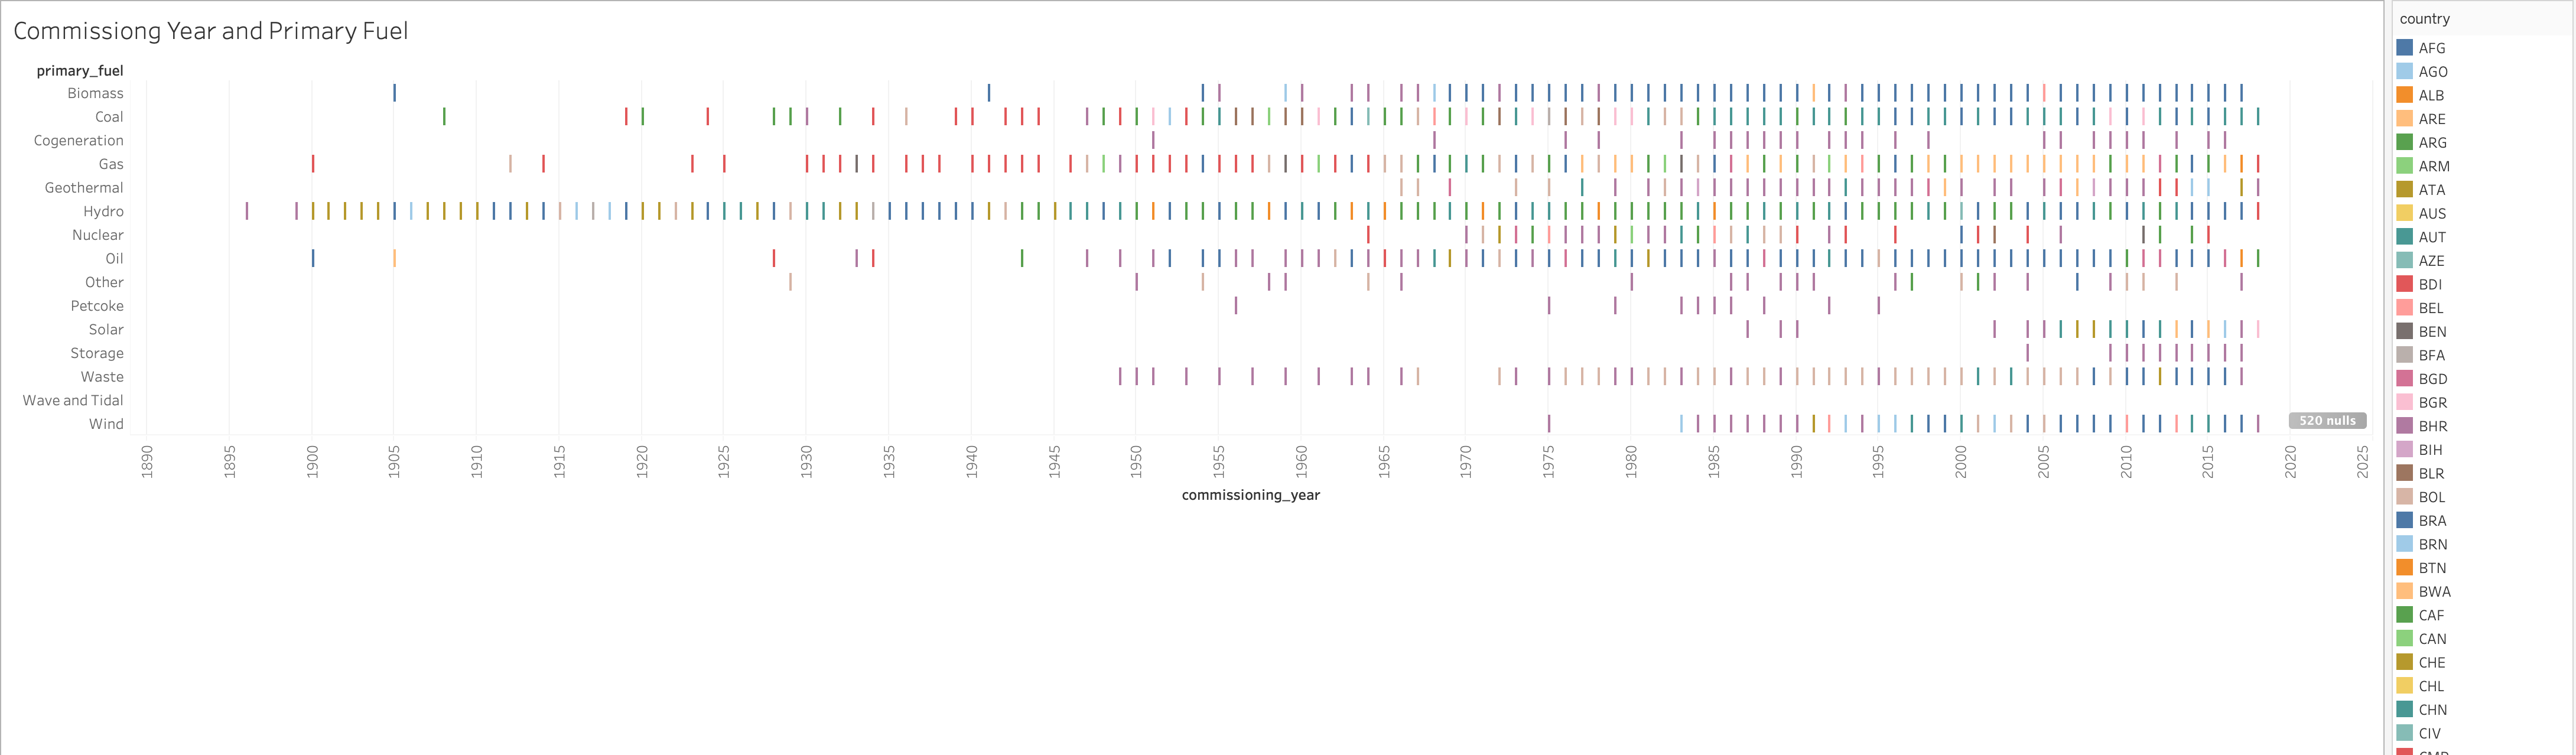
\includegraphics[width=15cm]{Viz1.png}

\hypertarget{description}{%
\subsubsection{Description}\label{description}}



\begin{description}
\item[Visual Design Type:]
Gantt
\item[Name of Tool:]
Tableua
\item[Country:]
All Countries
\item[Year:]
1896 - 2018
\item[Visual Mappings:]
\begin{itemize}
	\tightlist
	\item[  ]
\end{itemize}
\begin{itemize}
\tightlist
\item
  \textbf{mapping 1}: commissioning year x axis, y axis primary fuel.
\end{itemize}

\begin{itemize}
\tightlist
\item
  \textbf{mapping 2}: Country is used for the colouring of the points.
\end{itemize}
\item[Unique Observation:]
The oldest powerplant was commissioned in the USA in 1896 and its main fuel type was hydo. The second commissioned powerplant was also in the USA and again this was hydo which was commissioned in the 1899. Then in 1900 3 power plants were commissioned. These were Brazil with oil , Russia with gas and switzerland with hydro.

\item[Data Preparation:]
There was no modifications made to this dataset.
\end{description}
